
\chapter{MỞ ĐẦU}
\label{Introduction}

\section{Bối cảnh chung}


\begin{figure}[htbp]
	\centering
	\begin{subfigure}{0.35\textwidth}
		\centering
		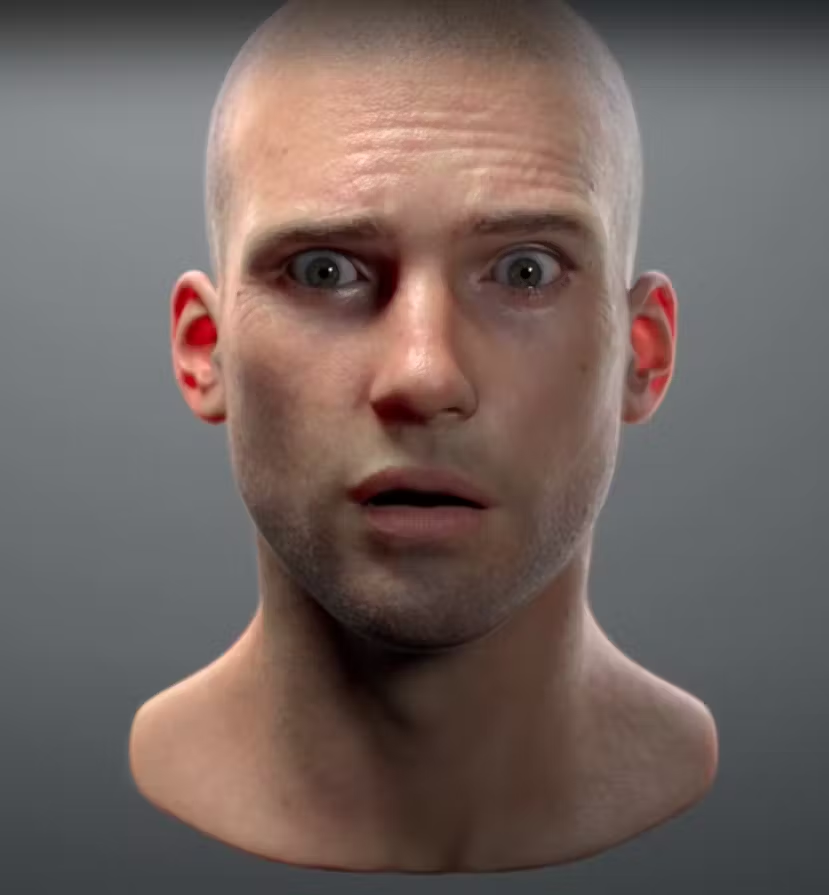
\includegraphics[height=5.8cm]{images/cgi}
		 \caption{\small Công nghệ CGI với người kỹ thuật số siêu thật \cite{edchrisjones}}
		\label{fig:CGI}
	\end{subfigure}
	\hfill
	\begin{subfigure}{0.6\textwidth}
		\centering
		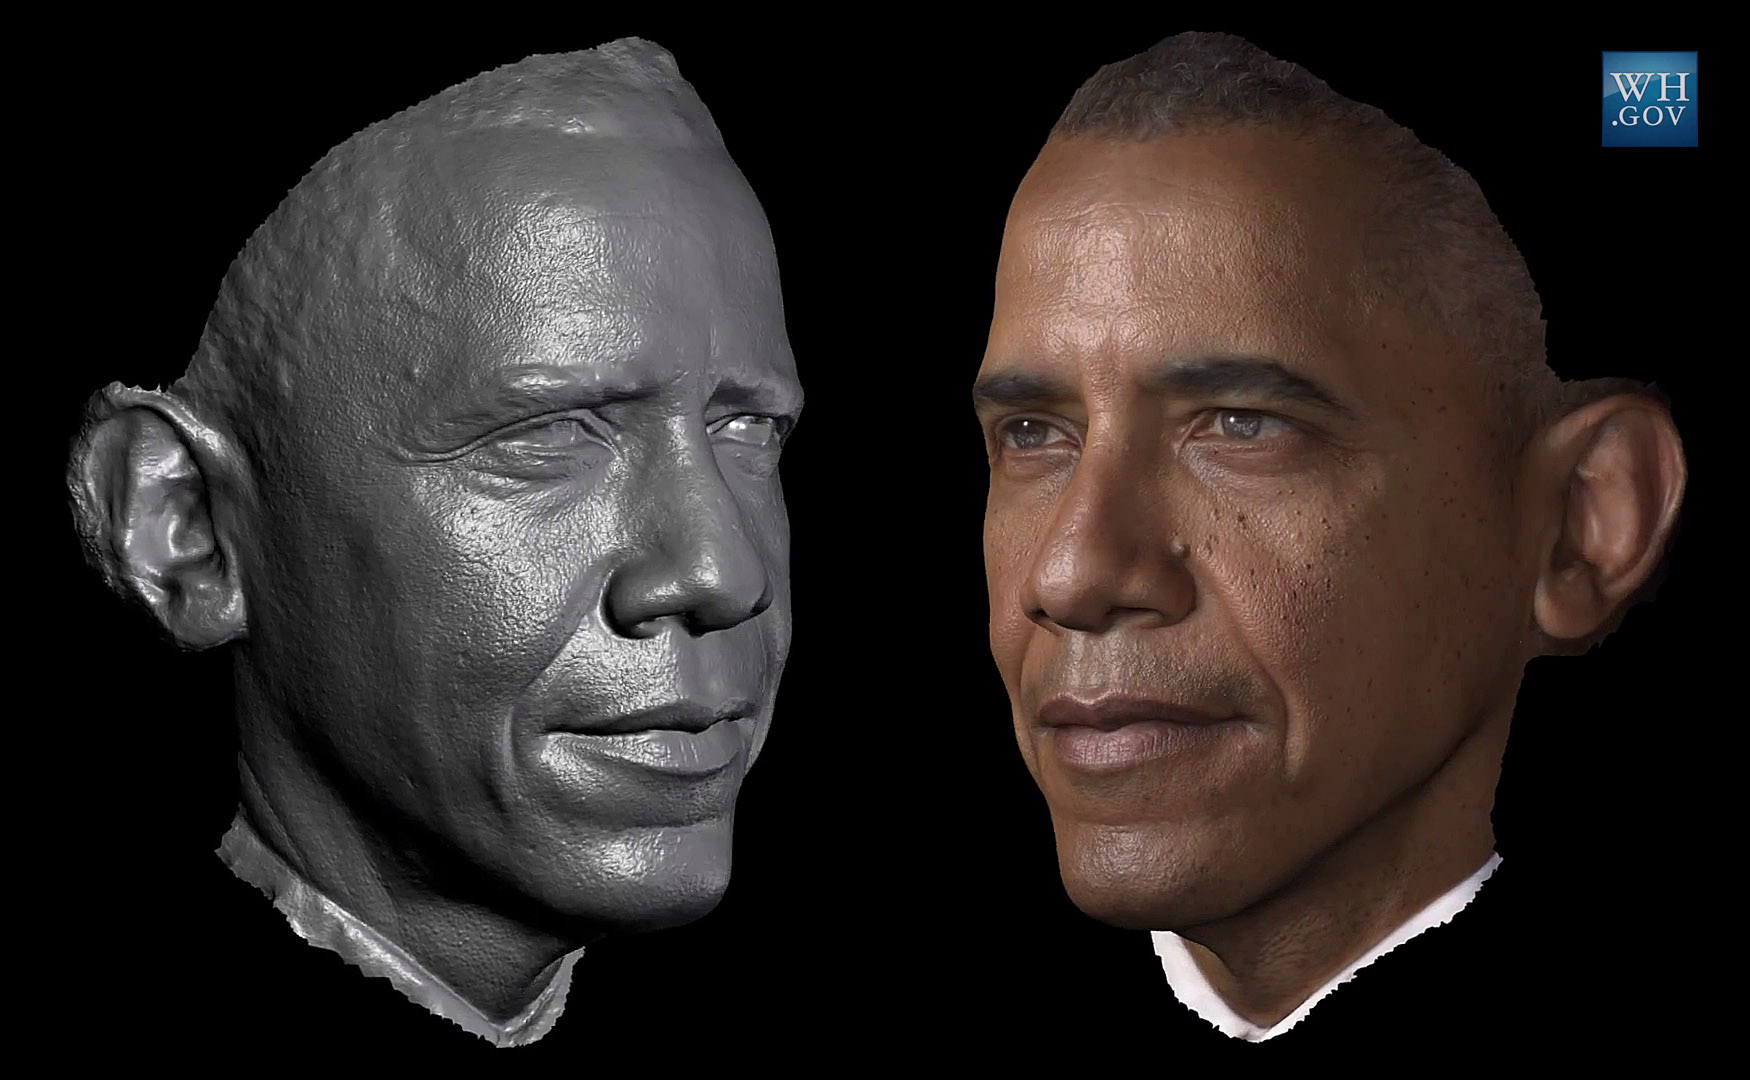
\includegraphics[height=5.8cm]{images/obama_scan}
		\caption{\small Minh họa công trình tái tạo khuôn mặt tổng thống Obama \cite{metallo2015scanning}}
		\label{fig:obamascan}
	\end{subfigure}
	\caption{Minh họa kỹ thuật đồ họa máy tính trong việc xây dựng người kỹ thuật số}
	\label{fig:DigitalHuman}
\end{figure}

Mỗi ngày, trên thế giới có hàng tỷ người nhìn vào màn hình RGB, kết quả hiển thị trên màn hình là đầu ra của mọi hệ thống phần mềm. Do đó, việc hiển thị từng pixel trên màn hình và cách để mô phỏng lại hình ảnh trên một cách chân thực nhất được các nhà khoa học về đồ họa máy tính (Computer Graphic) nghiên cứu từ những năm 1960s và đặc biệt là việc mô hình phỏng lại con người. Từ năm 2014, các họa sĩ 3D đã có thể tạo nên một nhân vật người siêu thật như \autoref{fig:CGI} trong khi đó các phần cứng máy tính còn chưa phát triển như hiện nay. 

Ngày nay, công nghệ đồ họa máy tính đã hoàn toàn có thể mô phỏng nhiều vật giống đến mức siêu thực (realistic), bao gồm các vật phức tạp như nước, đường xá, bánh mì,...  và thậm chí là cả cơ thể và khuôn mặt con người với độ chi tiết đến từng lông tơ, nốt mụn và vân mắt. 
Vào năm 2015, bằng kỹ thuật quét 3 chiều ghi lại toàn bộ các góc của khuôn mặt, sự phản chiếu ánh sáng, trong công trình \cite{metallo2015scanning}
các nhà khoa học đồ họa máy tính đã có thể tái tạo toàn bộ khuôn mặt của tổng thống Obama trên máy tính với độ chính xác cao và gần như không thể phân biệt \autoref{fig:obamascan}.

Trí tuệ nhân tạo thể hiện kết quả vượt bậc những năm gần đây, không chỉ trong nghiên cứu mà còn trong ứng dụng thực tế, tiêu biểu như ứng dụng ChatGPT, MidJourney và sự phát triển cả theo chiều dọc và chiều ngang trong nhiều lĩnh vực ứng dụng trí tuệ nhân tạo. Mặc dù đồ họa máy tính đã có thể xây dựng khuôn mặt người siêu thật, việc sinh cử chỉ lại phụ thuộc vào việc chụp chuyển động (Motion Capture) từ các cảm biến và gặp khó khăn khi xây dựng hệ thống trí tuệ nhân tạo học từ dữ liệu.

Các hệ thống trí tuệ nhân tạo hiện nay đã có thể tạo văn bản và giọng nói tiệm cận như con người, nhưng một trong những trở ngại lớn nhất để xây dựng con người kỹ thuật số hiện nay chính là việc sinh cử chỉ. Chính vì vậy, mục tiêu của luận văn là xây dựng một hệ thống sinh cử chỉ hội thoại dựa trên cảm xúc và ngữ nghĩa với dữ liệu đầu vào gồm cả văn bản và giọng nói.

\section{Động lực nghiên cứu}

Tổng hợp cử chỉ hội thoại giúp ích cho rất nhiều lĩnh vực như hoạt ảnh, dựng phim, trò chơi điện tử, giáo dục và những ứng dụng thực tế ảo. Việc tổng hợp cử chỉ chuyển động được thực hiện theo cách truyền thống là thuê các diễn viên sử dụng thiết bị theo dõi chuyển động và bố trí các hệ thống cảm biến xung quanh thu nhận chuyển động để đạt được độ chính xác chân thực nhất. Tuy nhiên, các chuyển động thu được sau đó chỉ được phát lại và không có sự biến đổi linh hoạt giữa các hành động. Do đó, việc áp dụng trí tuệ nhân tạo để có thể học các chuyển động từ dữ liệu thu nhận và sau đó có thể sinh ra dữ liệu mới sẽ là một cuộc cách mạng trong ngành công nghiệp chụp chuyển động.

Vào năm 2011, một nhóm tác giả \cite{bergmann2011relation} đã chứng minh rằng có sự liên hệ giữa giọng nói và cử chỉ con người, đây chính là tiền đề cho thấy chúng ta có thể dùng dữ liệu giọng nói để có thể dùng để học và biểu diễn được cử chỉ con người.
Với sự thành công của các mô hình ngôn ngữ tự nhiên trong xử lý văn bản và độ chính xác siêu thật trong việc mô phỏng gương mặt con người, ngành đồ họa máy tính đã đạt được những tiến bộ vượt bậc. Cùng với đó là sự dễ dàng và chính xác trong việc tổng hợp giọng nói con người.
Việc ứng dụng trí tuệ nhân tạo để sinh cử chỉ con người là một trong những điểm nghẽn chính trong phát triển trợ lý ảo giao tiếp và tương tác với con người.

\section{Dữ liệu bài toán}
\label{sec:Data}


\begin{figure}[H]
	\centering
	\begin{subfigure}{0.49\textwidth}
		\centering
		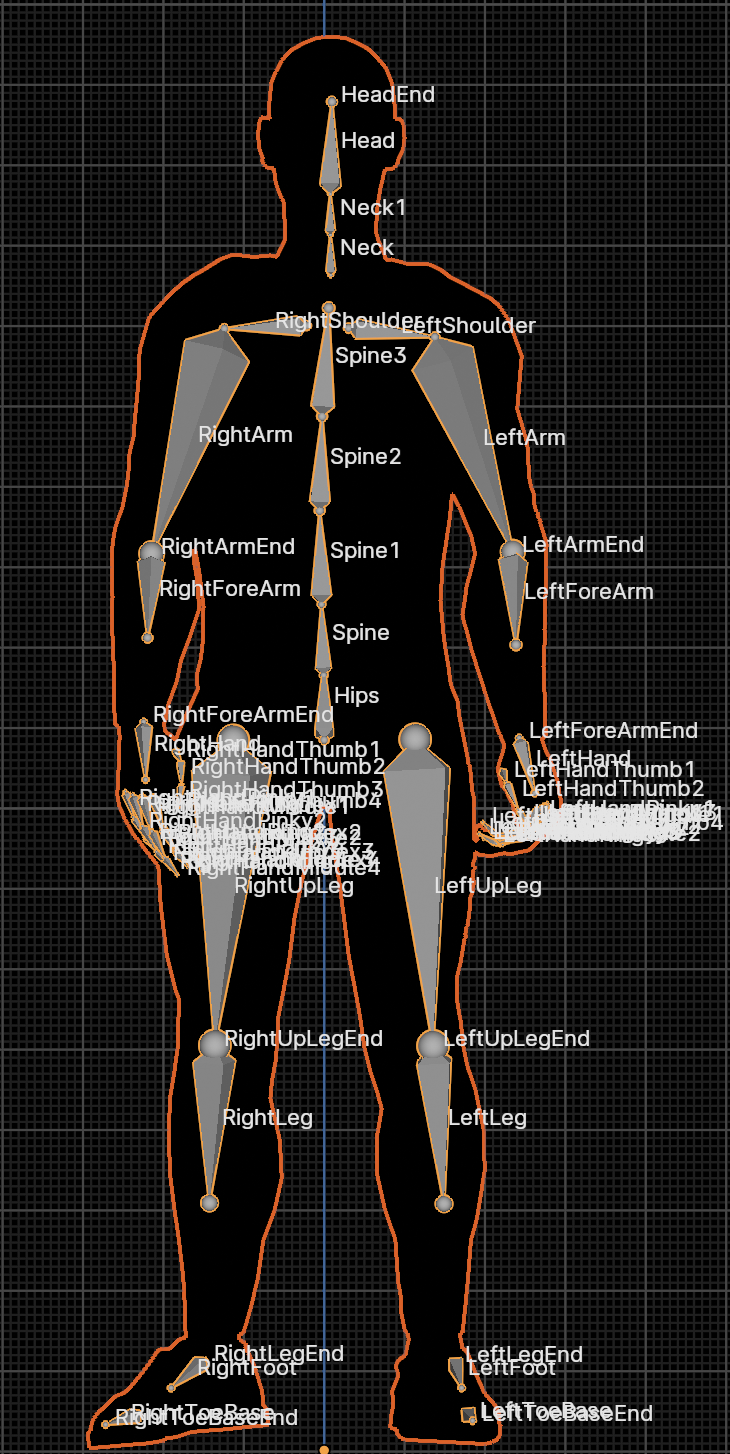
\includegraphics[height=10cm]{images/Skeleton.png}
		\caption{\small Khung xương và tên của các khớp của một khung xương trong mỗi khung hình.}
		\label{fig:Skeleton}
	\end{subfigure}
	\hfill
	\begin{subfigure}{0.49\textwidth}
		\centering
		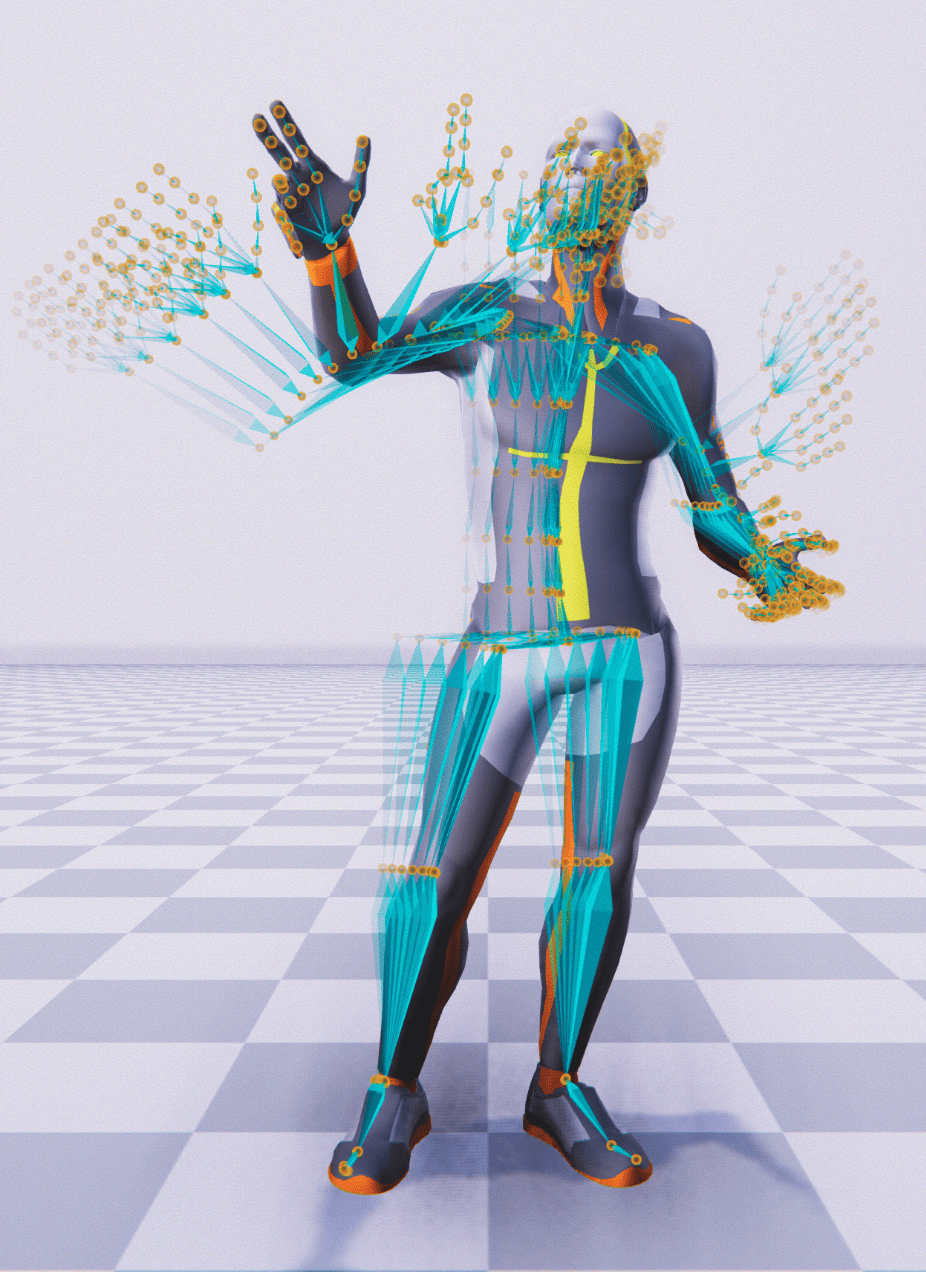
\includegraphics[height=10cm]{images/MotionPastAndFuture.png}
		\caption{\small Chuỗi chuyển động của cử chỉ bao gồm 6 cử chỉ quá khứ và 6 cử chỉ tương lai.}
		\label{fig:MotionPastAndFuture}
	\end{subfigure}
\end{figure}

\subsection{Kiến trúc khung xương của cử chỉ}

Cử chỉ (gesture) trong luận văn là sự chuyển động của toàn bộ cơ thể của một nhân vật như hình \autoref{fig:Skeleton} theo từng khung hình. Để có thể biểu diễn các chuyển động của một nhân vật trong đồ họa máy tính, các chuyển động sẽ được biểu diễn thành chuyển động của các xương (bone) riêng lẻ. Bao gồm cánh tay (hand), chân (leg), đầu (head), xương sống (spine),... Kiến trúc đầy đủ của một nhân vật được trình bày ở phụ lục \autoref{appendix:BVHData:skeleton}.

Dữ liệu một nhân vật theo thời gian trong thực tế sẽ được thu nhận bằng các hệ thống chụp chuyển động (motion capture) với các hệ thống camera và cảm biến chuyên biệt. Kết quả của quá trình motion capture là các tệp được định nghĩa dưới dạng tệp BVH (Biovision Hierarchy).

Các tệp BVH bao gồm hai thành phần chính: {HIERARCHY} và {MOTION}. HIERARCHY được thể hiện dưới dạng một cây bao gồm các thông tin về tên và vị trí khởi tạo các khung xương, MOTION là dữ liệu về chuyển động của toàn bộ khung xương theo từng khung hình (frame).  Mỗi tệp BVH sẽ có thông tin về số khung hình trên giây ($\text{fps}$) và tổng sống khung hình. Thông tin mỗi tệp BVH được trình bày ở phụ lục \autoref{appendix:BVHData:BVHStructure}. 


\subsection{Kiến trúc chuyển động của cử chỉ}

Dữ liệu chuyển động của cử chỉ như \autoref{fig:MotionPastAndFuture} hay phần MOTION của tệp BVH sẽ chứa thông tin về tọa độ và góc quay của một nhân vật theo từng khung hình. Dữ liệu mỗi khung hình là tập khung xương (skeleton) bao gồm $75$ xương (bone), $\{ \textbf{b}_{1}, \textbf{b}_{2}, \cdots , \textbf{b}_{75} \}$, mỗi xương thể hiện vị trí (position) $\{ p_{x}, p_{y}, p_{z} \}$ và góc quay (rotation) $\{ r_{x}, r_{y}, r_{z} \}$ chuyển động của một nhân vật theo thời gian.

Kết quả của việc sinh cử chỉ (gesture generation) là sinh ra chuỗi chuyển động góc quay các xương của nhân vật theo từng khung hình (frame). Việc sinh cử chỉ (gesture generation) được đánh giá bằng việc tạo ra các cử chỉ tự nhiên, giống con người (human-likeness) và phù hợp với ngữ cảnh.

Trong luận văn, các dữ liệu về vị trí và góc quay của khung xương nhân vật được tiền xử lý để chuyển thành một vector đặc trưng $\mathbf{g} \in \mathbb{R}^{D}$ với $D=1141$. Dữ liệu cần học khi đó sẽ là $\bx \in \mathbb{R}^{M \times D}$.

Quá trình xử lý dữ liệu được trình bày đầy đủ ở \autoref{appendix:BVHData}.

\section{Phát biểu bài toán}
\label{sec:ProblemStatement}

Với kết quả cuối cùng là chuỗi cử chỉ thể hiện sự chuyển động của các khung xương theo từng khung hình, thì có rất nhiều phương pháp khác nhau như phương pháp học phân loại (classification), gom nhóm (clustering), hồi quy (regression), .. . Trong luận văn này, sinh cử chỉ là  được cho bài toán hồi quy (regression), tạo ra dữ liệu mới dựa trên mô hình sinh, với đầu vào là một chuỗi cử chỉ cho trước và đầu ra là chuỗi cử chỉ tiếp theo cần dự đoán.
	
\begin{figure}[H]
	\centering
	\href{https://www.youtube.com/watch?v=B6nv1kQmi-Q}{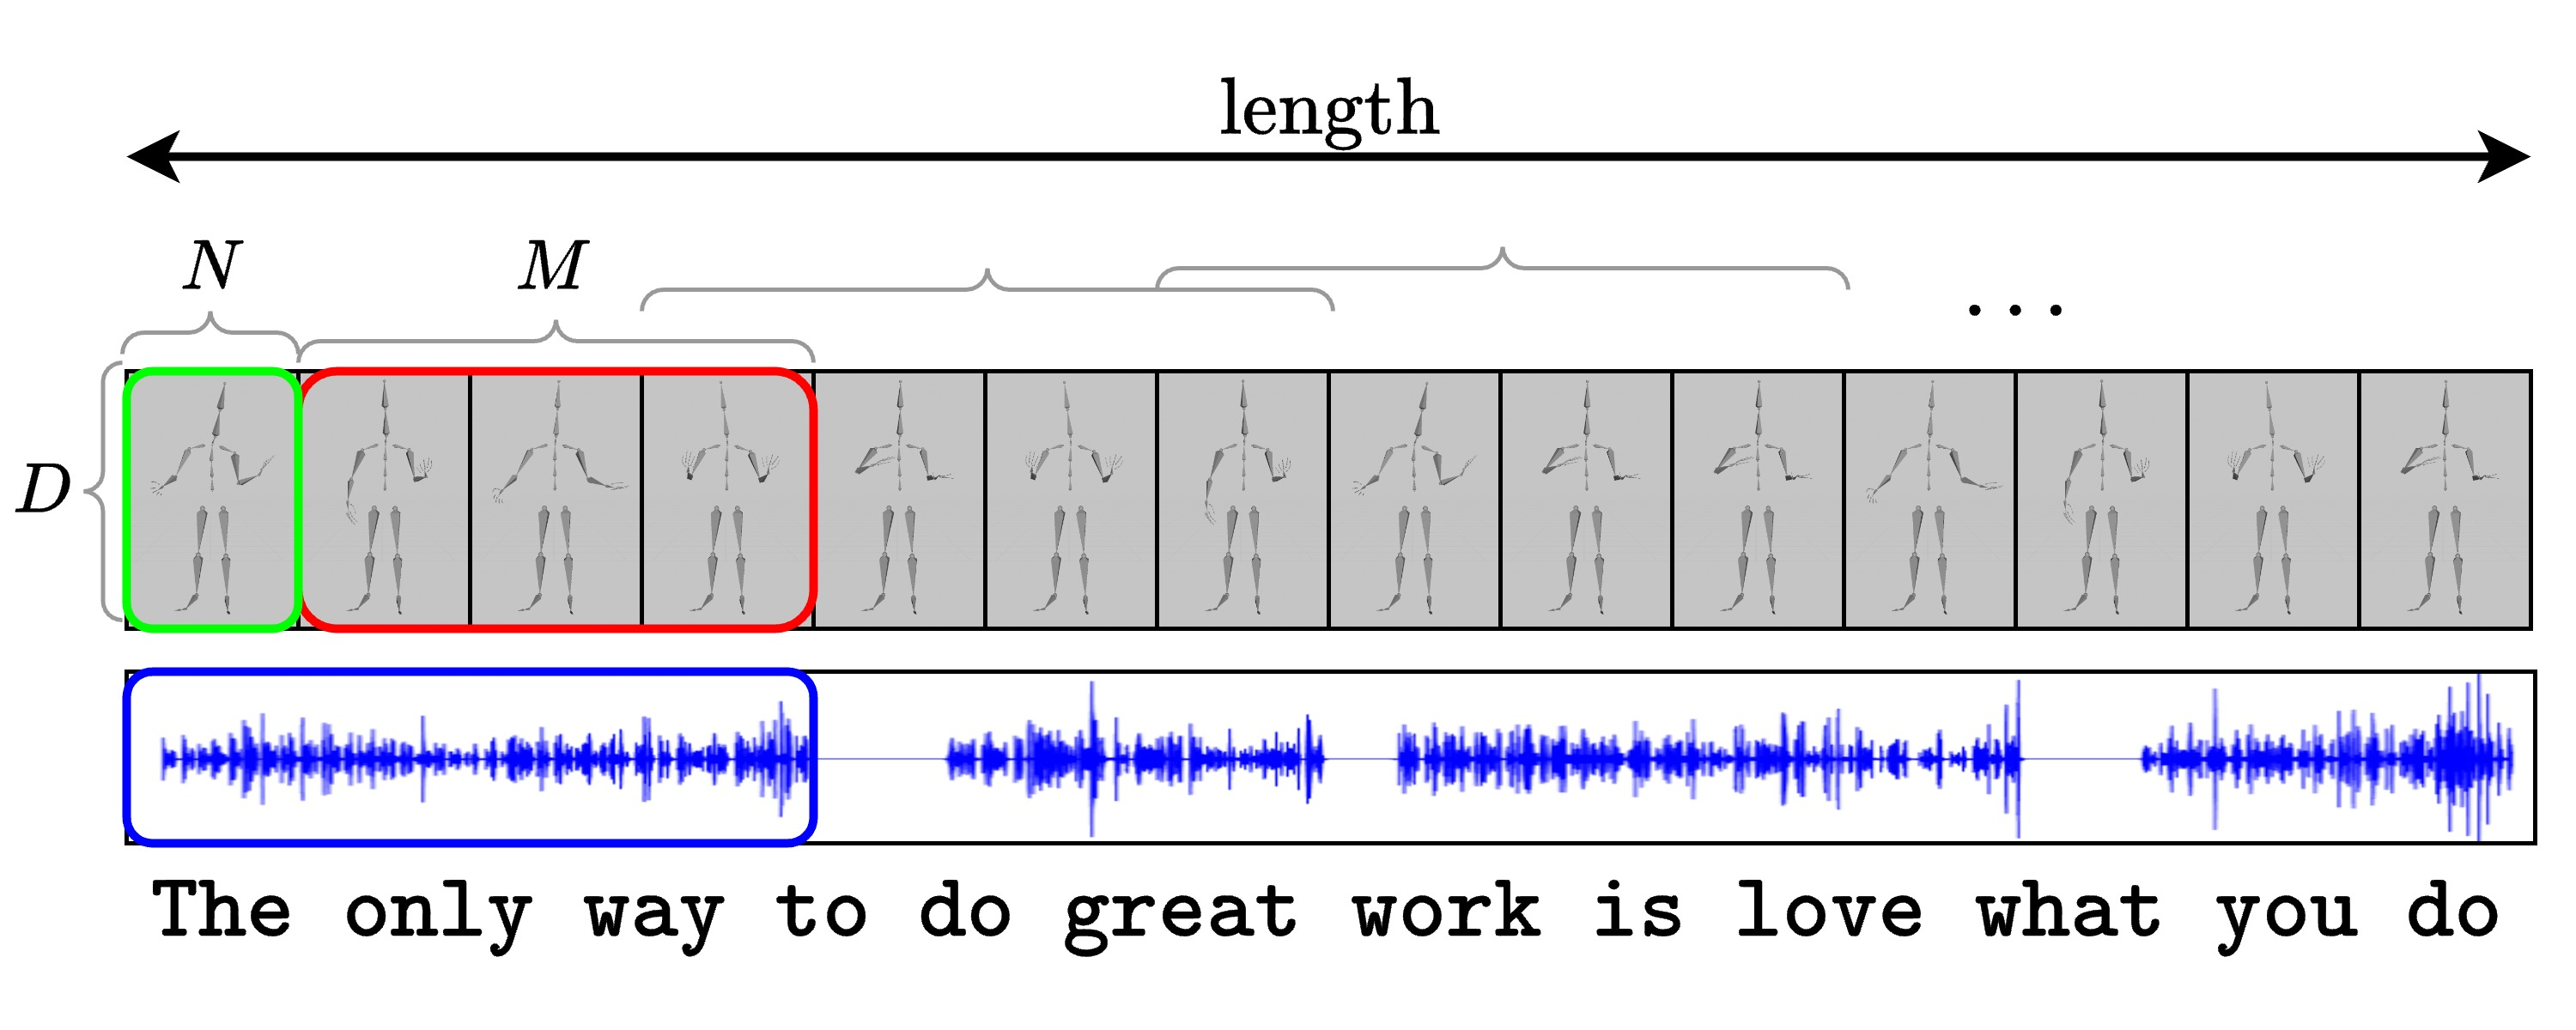
\includegraphics[width=\linewidth]{FeatureProcessing}}
	\caption{Minh họa một chuỗi cử chỉ, $N$ frame đầu được lấy làm cử chỉ khởi tạo $\mathbf{s}$ (seed gesture) và $M$ khung hình còn lại làm cử chỉ để học}
	\label{fig:GestureSeries}
\end{figure}

Với một chuỗi cử chỉ có độ dài khung hình bất kỳ, cảm xúc sẽ được gán cho toàn bộ chuỗi cử chỉ. Một phần cải tiến của luận văn là tương ứng với chuỗi cử chỉ là dữ liệu giọng nói và đoạn văn bản được dịch từ dữ liệu giọng nói tương ứng.
Mục tiêu của luận văn là xây dựng mô hình để dự đoán từng đoạn nhỏ, với thông tin dữ liệu đầu vào bao gồm chuỗi $N$ frame cử chỉ cho trước $\mathbf{s} \in \mathbb{R}^{1:N \times D}$ (seed gesture), chuỗi giọng nói $\mathbf{a}$ (speech), văn bản $\mathbf{v}$ (text),  cảm xúc $\mathbf{e}$ (emotion) tương ứng.

Kết quả dự đoán của mô hình là $\hat{\mathbf{x}} \in \mathbb{R}^{1:M \times D}$ bao gồm từ frame 1 đến frame $M$ chuỗi cử chỉ tiếp theo . Với dữ liệu gốc là chuỗi cử chỉ đã có $\mathbf{x}  \in \mathbb{R}^{1:M \times D}$.

\begin{multicols}{2}
	
\textbf{Đầu vào}

\begin{itemize}
	\item Chuỗi cử chỉ khởi tạo: $\mathbf{s} \in \mathbb{R}^{1:N \times D}$
	\item Chuỗi giọng nói: $\mathbf{a}$
	\item Văn bản: $\mathbf{v}$ 
	%				\in \mathbb{R}^{16000 M}
	%			trích xuất đặc trưng MFCC: $\mathbf{a} \in \mathbb{R}^{M \times C_{\text{mfcc}}}$
	\item Cảm xúc: $\mathbf{e}$ 
	
	{\small
		(\texttt{Happy},  \texttt{Sad},  \texttt{Neutral}, \texttt{Angry}, \texttt{Old}, \texttt{Funny})
	}
\end{itemize}

\columnbreak

\textbf{Dữ liệu dự đoán}
\vspace{-10pt}
\begin{itemize}
	\item Chuỗi cử chỉ dự đoán: $\hat{\mathbf{x}} \in \mathbb{R}^{1:M \times D}$
\end{itemize}

\textbf{Dữ liệu gốc}
\vspace{-10pt}
\begin{itemize}
	\item Chuỗi cử chỉ gốc: $ \mathbf{x}  \in \mathbb{R}^{1:M \times D}$
\end{itemize}

\end{multicols}

\section{Các khó khăn cần giải quyết}
\label{sec:difficult}

Có rất nhiều khó khăn trong việc xây dựng một mô hình có thể học được các đặc trưng cử chỉ hội thoại như con người.

Thứ nhất, \textit{dữ liệu không đủ nhiều và chất lượng}, chi phí để tạo ra một bộ dữ liệu trong ngành công nghiệp chụp chuyển động có chất lượng và quy mô lớn để ứng dụng thực tế là rất cao.

Thứ hai, \textit{sự thiếu đồng nhất về ngữ cảnh của các loại dữ liệu}, các bộ dữ liệu về văn bản thường nhiều hơn so với giọng nói, và cũng không rõ văn bản đó được tạo ra bởi ai. Sự đồng bộ giữa giọng nói và cảm xúc khi nói cũng thường thiếu trong tập dữ liệu. Ngoài ra, dữ liệu văn bản trong tập dữ liệu huấn luyện lại thuộc nhiều chủ đề đa dạng.
 
Thứ ba, \textit{sự phân bố không cân xứng về  dữ liệu giữa các loại đặc trưng cần học}. Các dữ liệu dùng cho nghiên cứu cử chỉ hiện nay thường tập trung vào ngôn ngữ Tiếng Anh, các cử chỉ có sự phân bố không cân xứng giữa các trạng thái như nói, hỏi, hoặc im lặng.

Thứ tư, \textit{chi phí tính toán với nhiều loại dữ liệu của mô hình là một thách thức lớn}. Với đầu vào của mô hình gồm nhiều loại dữ liệu như văn bản, tiếng nói và điểm 3D, cần nhiều lớp mã hóa cho từng loại dữ liệu, dẫn đến chi phí tính toán cao trong cả giai đoạn huấn luyện và suy luận. Nếu giảm thông tin dữ liệu đầu vào cũng sẽ giảm kết quả suy luận của mô hình khi sinh cử chỉ.

Cuối cùng, \textit{các bước xử lý cần được thực hiện tuần tự}, cách hiệu quả nhất để con người tương tác với máy tính là thông qua giọng nói và nhập từ bàn phím, tuy nhiên việc xử lý được văn bản và giọng nói để làm đầu vào cho mô hình phải thực hiện tuần tự. Độ trễ trong quá trình suy luận của sản phẩm thực tế cũng là một vấn đề lớn, vì người dùng không thể chờ đợi quá lâu để nhận kết quả. Ngoài ra, việc hiển thị cử chỉ đó lên máy tính bằng kỹ thuật đồ họa cũng cần được tối ưu để giảm thời gian xử lý.


\section{Đóng góp dự kiến}

\begin{itemize}
	\item Dựa trên tập dữ liệu có sẵn, luận văn chuyển giọng nói trong tập dữ liệu thành văn bản, và dùng văn bản đó để làm dữ liệu huấn luyện mới như là một dữ liệu ngữ nghĩa bổ sung trong quá trình học.
	
	\item Dựa trên mô hình cơ bản DiffuseStyleGesture, luận văn mở rộng thêm đặc trưng văn bản trong quá trình khử nhiễu có điều kiện.
	
	\item Luận văn sử dụng Unity để render, trích xuất dữ liệu và trực quan hóa kết quả sinh cử chỉ.
	
	\item Luận văn xây dựng hệ thống kết xuất, và minh họa chương trình bằng Unity
\end{itemize}


% Ngôn ngữ để viết và trình bày báo cáo khóa luận tốt nghiệp, đồ án tốt nghiệp, thực tập tốt nghiệp (sau đây gọi chung là báo cáo) là tiếng Việt hoặc tiếng Anh. 
% Trường hợp chọn ngôn ngữ tiếng Anh để viết và trình bày báo cáo,  sinh viên cần có đơn đề nghị, được cán bộ hướng dẫn (CBHD) đồng ý và nộp cho bộ phận Giáo vụ của Khoa vào thời điểm đăng ký đề tài để xin ý kiến.
% Báo cáo viết và trình bày bằng tiếng Anh phải có bản tóm tắt viết bằng tiếng Việt.


%Tóm tắt luận văn được trình bày nhiều nhất trong 24 trang in trên hai mặt giấy, cỡ chữ Times New Roman 11 của hệ soạn thảo Winword hoặc phần mềm soạn thảo Latex đối với các chuyên ngành thuộc ngành Toán.

%Mật độ chữ bình thường, không được nén hoặc kéo dãn khoảng cách giữa các chữ.
%Chế độ dãn dòng là Exactly 17pt.
%Lề trên, lề dưới, lề trái, lề phải đều là 1.5 cm.
%Các bảng biểu trình bày theo chiều ngang khổ giấy thì đầu bảng là lề trái của trang.
%Tóm tắt luận án phải phản ảnh trung thực kết cấu, bố cục và nội dung của luận án, phải ghi đầy đủ toàn văn kết luận của luận án.
%Mẫu trình bày trang bìa của tóm tắt luận văn (phụ lục 1).
